\documentclass{ctexart}
\usepackage{tikz}
\begin{document}
% 1.字符串变量
%   \def<register>{<str>}
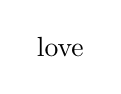
\begin{tikzpicture}
    \def\mstrv{love}
    \node at (0,0){\mstrv};
\end{tikzpicture}



% 2.数学表达式(取结果)变量. section 94
%   1)\pgfmathparse{<expression>}
%     将表达式的结果赋予宏\pgfmathresult, 并且紧跟\pgfmathresult进行宏引用. 即\pgfmathparse{<expression>}\pgfmathresult一体
%     在表达式中,遵循以下规则:
%       [1]将字符串视为function名称
%       [2]""内的内容视为字符串
%       [3]将数字全部转化为以pt为单位(数值进行单位转换,而非只换单位),没有带单位的默认为pt;进行计算;结果截去单位,为纯数字
%       [4]可识别TeX register
%     {<expression>}为\pgfmathparse{<expression>}\pgfmathresult的缩写形式
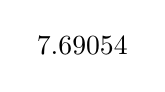
\begin{tikzpicture}
    \node at (0,0){\pgfmathparse{2pt+2mm}\pgfmathresult};
\end{tikzpicture}

%   2)\pgfmathsetmacro{<macro>}{<expression>}
%     将\pgfmathparse结果赋予指定宏
%     宏为以\开头的引用变量
%     数字结果为纯数字,不带单位
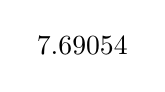
\begin{tikzpicture}
    \pgfmathsetmacro{\mre}{2pt+2mm}
    \node at (0,0){\mre};
\end{tikzpicture}

%   3)\pgfmathsetlengthmacro{<macro>}{<expression>}
%     将\pgfmathparse结果赋予指定宏
%     宏为以\开头的引用变量
%     结果为带pt单位的数字
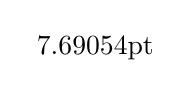
\begin{tikzpicture}
    \pgfmathsetlengthmacro{\mre}{2pt+2mm}
    \node at (0,0){\mre};
\end{tikzpicture}

%   4)\pgfmathtruncatemacro{<macro>}{<expression>}
%     将\pgfmathparse结果,截取整数部分后赋予指定宏
%     宏为以\开头的引用变量
%     结果为纯数字,不带单位
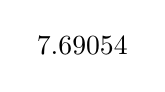
\begin{tikzpicture}
    \pgfmathsetmacro{\mre}{2pt+2mm}
    \node at (0,0){\mre};
\end{tikzpicture}

%   5)\pgfmathsetlength{<register>}{<expression>}
%     将\pgfmathparse结果赋予指定tex register
%     tex register为以\开头的引用变量
%     tex register引用方式: \the<register>
%     tex register带pt单位
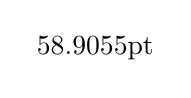
\begin{tikzpicture}
    \dimendef\mre=0
    \pgfmathsetlength{\mre}{2pt+2cm}
    \node at (0,0){\the\mre};
\end{tikzpicture}

%   6)\pgfmathaddtolength{<register>}{<expression>}
%     将\pgfmathparse结果与tex register的原内容相加,并赋予tex register
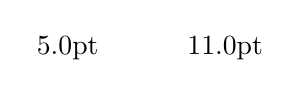
\begin{tikzpicture}
    \dimendef\mre=0
    \pgfmathsetlength{\mre}{2pt+3pt}
    \node at (0,0){\the\mre};
    \pgfmathaddtolength{\mre}{6pt}
    \node at (2,0){\the\mre};
\end{tikzpicture}

%   7)\pdfmathsetcount{<count_register>}{<expression>}
%     将\pgfmathparse结果,截取整数部分,赋予指定tex count register
%     tex count resgister为纯数字,不带单位
\begin{tikzpicture}
    \newcount\mcou
    \pgfmathsetcount{\mcou}{2pt+2mm}
    \node at (0,0){\the\mcou};
\end{tikzpicture}

%   8)\pgfmathaddtocount{<count_register>}{<expression>}
%     将\pgfmathparse结果与tex count register的原内容相加,并赋予tex count register
\begin{tikzpicture}
    \newcount\mcou
    \pgfmathsetcount{\mcou}{2pt+2mm}
    \node at (0,0){\the\mcou};
    \pgfmathaddtocount{\mcou}{6pt}
    \node at (2,0){\the\mcou};
\end{tikzpicture}

%   9)\pgfmathdeclarerandomlist{<list_name>}{{<item_1>}{<item_2>}...}
%     生成一个数组,指定数组的item

%   10)\pgfmathrandomitem{<macro>}{<list_name>}
%     从数组中随机选择一个数,保存到指定宏
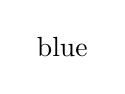
\begin{tikzpicture}
    \pgfmathdeclarerandomlist{minelist}{{red}{green}{blue}{orangle}}
    \pgfmathrandomitem{\myself}{minelist}
    \node at (0,0){\myself};
\end{tikzpicture}

% 整数之间的转化
%   11)\pgfmathbasetodec{<macro>}{<number>}{<base>}
%     将进制为base的数字number转化为10进制,并赋予macro

%   12)\pgfmathdectobase{<macro>}{<number>}{<base>}
%     将10进制数字number转化为base进制,并赋予macro
%     结果字母都为小写

%   13)\pgfmathdectoBase{<macro>}{<number>}{<base>}
%     将10进制数字number转化为base进制,并赋予macro
%     结果字母都为大写

%   14)\pgfmathbasetobase{<macro>}{<number>}{<base_1>}{<base_2>}
%     将base_1进制数字number转化为base_2进制数字,并赋予macro
%     结果字母都为小写

%   15)\pgfmathbasetoBase{<macro>}{<number>}{<base_1>}{<base_2>}
%     将base_1进制数字number转化为base_2进制数字,并赋予macro
%     结果字母都为大写

%   16)\pdfmathsetbasenumberlength{<length>}
%     指定整数之间转化,结果的位数

%   17)\pgfmathtodigitlist{<macro>}{<number>}
%     将数字number添加到数组macro中
\begin{tikzpicture}
    \foreach \in in {1,2,...,8}
      \pgfmathtodigitlist{\mylist}{\in}
    \foreach \out in \mylist
      \node at (\out,0){\out};
\end{tikzpicture}


% 角度计算
%   18)\pgfmathanglebetweenpoints{<p>}{<q>}
%     水平线到p--q线的偏转角度. 值域范围[0,360]
%     坐标点使用\pgfpoint{<x_dimension>}{<y_dimension>}
%     结果保存在\pgfmathresult


%   19)\pgfmathanglebetweenlines{<p>}{<q>}{<m>}{<n>}
%     线条p--q到m--n的偏转角度. 值域范围[0,360]
%     坐标点使用\pgfpoint{<x_dimension>}{<y_dimension>}
%     结果保存在\pgfmathresult


% \pgfmathparse可识别运算:
%    数学运算:
%    x + y
%      x与y相加
%     
%    x - y
%      x减去y

%    -x
%      x的相反数

%    x * y
%      x乘以y

%    x / y
%      x除以y

%    x ^ y
%      x的y次方

%    x!
%      x的阶乘
%    x r
%      将弧度(pi)转化为角度(180)
%      
%    x ? y : z
%      三元运算符,if x then y else z

%    逻辑运算(true返回1,false返回0):
%    x == y
%      x是否等于y
%      
%    x > y
%      x是否大于y
%      
%    x < y
%      x是否小于y
%      
%    x != y
%      x是否不等于y
%    
%    x >= y
%      x是否大于等于y
%      
%    x <= y
%      x是否小于等于y
%    
%    x && y
%      与运算符
%      
%    x || y
%      或运算符
%      
%    !x
%      x的非运算

%    ()
%      优先级运算符
%      
%    {}
%      数组
%      
%    []
%      数组索引
%      
%    "x"
%      限定x为逐字符字符串
%      但可以使用以\开头的命令


%    常量:
%    e
%      自然数2.718281828

%    pi
%      3.141592654

%    rnd
%      符合统一分布的伪随机数,范围[0,1]

%    rand
%      符合统一分布的伪随机数,范围[-1,1]

%    
%    函数:
%    div(x,y)
%      x除以y,并只取结果的整数部分

%    sqrt(<num>)
%      求平方根

%    exp(x)
%      求e^x

%    ln(x)
%      以e为底数的对数

%    log2(x)
%      以2为底数的对数

%    log10(x)
%      以10为底数的对数

%    abs(x)
%      求绝对值

%    mod(x,y)
%      求x除以y的余数. 结果符号与x/y一致

%    Mod(x,y)
%      求x除以y的余数. 结果符号恒为正

%    sign(x)
%      取x的正负. 正为1,0为0,负为-1

%    round(x)
%      四舍五入取整数

%    floor(x)
%      向下取整数

%    ceil(x)
%      向上取整数

%    int(x)
%      截取整数部分

%    frac(x)
%      截取小数部分

%    real(x)
%      返回小数形式的数字

%    gcd(x,y)
%      x/y的最大公约数

%    isodd(x)
%      检查x的整数部分是否为奇数

%    iseven(x)
%      检查x的整数部分是否为偶数

%    isprime(x)
%      检查x的整数部分是否为质数

%    rad(x)
%      将角度转化为弧度

%    deg(x)
%      将弧度转化为角度

%    sin(x)
%      求正弦值
%      x需要为角度值

%    cos(x)
%      求余弦值

%    tan(x)
%      求正切值

%    sec(x)
%    cosec(x)

%    cot(x)
%      求余切值

%    asin(x)
%      求反正弦值, 值域[-90,90]
%      返回值为角度值  
%    
%    acos(x)
%      求反余弦值,值域[0,180]

%    atan(x)
%      求反正切值

%    atan2(y,x)
%      求y/x的反正切值

%    /pgf/trig format=deg | rad
%    三角函数的参数视为角度还是弧度,默认为deg
%    \pgfkeys{/pgf/trig format=rad}


%    random(x,y)
%      该函数有三种格式. 格式如下:
%        1)random() - 符合统一分布的数字,区间[0,1]
%	2)random(x) - 符合统一分布的数字,区间[1,x]的整数
%	3)random(x,y) - 符合统一分布的数字,区间[x,y]的整数


%    hex(x)
%      将10进制数字转化为16进制. 字母部分为小写数字

%    Hex(x)
%      将10进制数字转化为16进制. 字母部分为大写数字

%    oct(x)
%      将10进制数字转化为8进制

%    bin(x)
%      将10进制数字转化为2进制

%    min(x1,x2,...,xn)
%      求数字的最小值

%    max(x1,x2,...,xn)
%      求数字的最大值
%    
%    veclen(<len_x>,<len_y>)
%      求长度sqrt(x^2+y^2)

%    array(x,y)
%      返回数组x的索引y
%      索引从0起始

%    dim(x)
%      返回数组的长度

%    sinh(x)
%      双曲正弦函数. (e^x - e^(-x)) / 2

%    cosh(x)
%      双曲余弦函数. (e^x + e^(-x)) / 2

%    tanh(x)
%      双曲正切函数. (e^x - e^(-x)) / (e^x + e^(-x))

%    width("x")
%      指定字符串的长度

%    height("x")
%      指定字符串的高度

%    depth("x")
%      指定字符串的深度
\end{tikzpicture}

% update by 2025-04-24
\end{document}

